\documentclass{article}

% Language setting
% Replace `english' with e.g. `spanish' to change the document language
\usepackage[english]{babel}

% Set page size and margins
% Replace `letterpaper' with `a4paper' for UK/EU standard size
\usepackage[letterpaper,top=2cm,bottom=2cm,left=3cm,right=3cm,marginparwidth=1.75cm]{geometry}

% Useful packages
\usepackage{amsmath}
\usepackage{graphicx}
\usepackage{amssymb}
\usepackage{array}
\usepackage[colorlinks=true, allcolors=blue]{hyperref}

\title{Finch: A Datastructure-Driven Array Programming Language}
\author{Willow Ahrens, Teo Collins, Radha Patel, Changwan Hong, Saman Amarasinghe}

\begin{document}
\maketitle

\begin{abstract}
From FORTRAN to Numpy, arrays have revolutionized how we express computation.
Arrays are the highest-performing datastructure with a long history of investment and innovation, from hardware support to compiler technology. 
However, arrays can only handle dense rectilinear integer grids. Real world arrays often contain underlying structure, such as sparsity, runs of repeated values, or symmetry. We describe a compiler, Finch, which adapts existing programs and interfaces to the structure and sparsity of the inputs. Finch enables programmers to capture complex, real-world data scenarios with the same productivity they expect from dense arrays. Our approach enables new loop optimizations across multiple domains, unifying techniques such as sparse tensors, databases, and lossless compression. 
\end{abstract}

\section{Introduction}

- Fortran supported lots of control structures, no data structures, just dense arrays.

- We tried to emulate complex data using only dense arrays but with complicated control structures.

- Recently, people tried to build frameworks to support structured data, but gave up a lot of program side

- We’re bringing these together, both need to work together.

\subsection{Contributions}

\begin{enumerate}
\item A complete set of level formats for expressing data patterns hierarchically in FiberTree-style decompositions. The first such set of formats to efficiently capture banded, triangular, run-length-encoded, or sparse-run-length-encoded datasets. The formats capture many use cases, from random updates to sequential construction.
\item The Finch array language, mirroring simple for-loops with imperative code blocks and if-conditions. The first array programming language for the above data formats to support multiple outputs, affine indexing, and imperfectly-nested loops.
\item Tensor lifecycles, a simple constraint on tensor reads and writes that elegantly restricts Finch programs to avoid complex data dependencies, and enables tensor polymorphism by providing implementers with well-defined functions to overload.
\item Wrapper Tensors which modify existing datastructures and recombine them to support new patterns, such as affine indexing, padding, transposition, and slicing.
\item Wrapper Levels which modify existing datastructures and enabling complex features such as atomic updates or contiguous versus separate allocation.
\item We define the first mappings from the existing pydata/sparse array api high-level operations to low level finch notation
\item <Performance Contributions>
\end{enumerate}

\begin{table}[h!]
\centering
\begin{tabular}{l|ccccc}
\textbf{Feature / Tool} & \textbf{Halide} & \textbf{Taco} & \textbf{Cora} & \textbf{Taichi} & \textbf{Finch} \\
\hline
Einsums and Contractions & \checkmark & \checkmark & \checkmark & \checkmark & \checkmark \\
Parallelism             & \checkmark & \checkmark & \checkmark & \checkmark & \checkmark \\
Multiple LHS            & \checkmark &            & \checkmark & \checkmark & \checkmark \\
Affine Indices          & \checkmark &            &            & \checkmark & \checkmark \\
Recurrence              & \checkmark &            &            &            &            \\
If-Conditions and Masks & \checkmark & \checkmark &            & \checkmark & \checkmark \\
Scatter Gather          & \checkmark &            &            & \checkmark & \checkmark \\
Early Break             &            & \checkmark &            &   \checkmark         & \checkmark \\
\end{tabular}
\caption{Feature support across various tools.}
\label{tab:features}
\end{table}

\begin{table}[h!]
\centering
\begin{tabular}{l|ccccc}
\textbf{Feature / Tool} & \textbf{Halide} & \textbf{Taco} & \textbf{Cora} & \textbf{Taichi} & \textbf{Finch} \\
\hline
Dense                    & \checkmark & \checkmark & \checkmark & \checkmark & \checkmark \\
Padded                   & \checkmark &            &            &            & \checkmark \\
One Sparse               &            & \checkmark &            & \checkmark & \checkmark \\
Sparse                   &            & \checkmark &            &            & \checkmark \\
Run-length               &            &            &            &            & \checkmark \\
Symmetric                &            &            &            &            & \checkmark \\
Regular Sparse Blocks    &            & \checkmark &            &            & \checkmark \\
Irregular Sparse Blocks  &            &            &            &            & \checkmark \\
Ragged                   &            &            & \checkmark &            & \checkmark \\
\end{tabular}
\caption{Support for various data structures across tools.}
\label{tab:data_structures}
\end{table}

\section{Additional Topics}

\begin{enumerate}
\item Concordant iteration
\item Dimensionalization
\item Bounds analysis/queries
\item Performance warnings

\end{enumerate}

\section{Evaluation}

\subsection{Data-Driven Performance Engineering}
\subsubsection{Sparse-Sparse Matrix Multiply}
Examples that demonstrate performance engineering in a datastructure-driven model

\subsubsection{SpMV}

%Here's a figure with spmv_performance_sorted_(faster_than_taco).png and spmv_performance_sorted_(slower_than_taco).png

\begin{figure}
    \begin{minipage}[t]{0.5\textwidth}
        \vspace{0pt} % Add this to ensure top alignment within minipage
        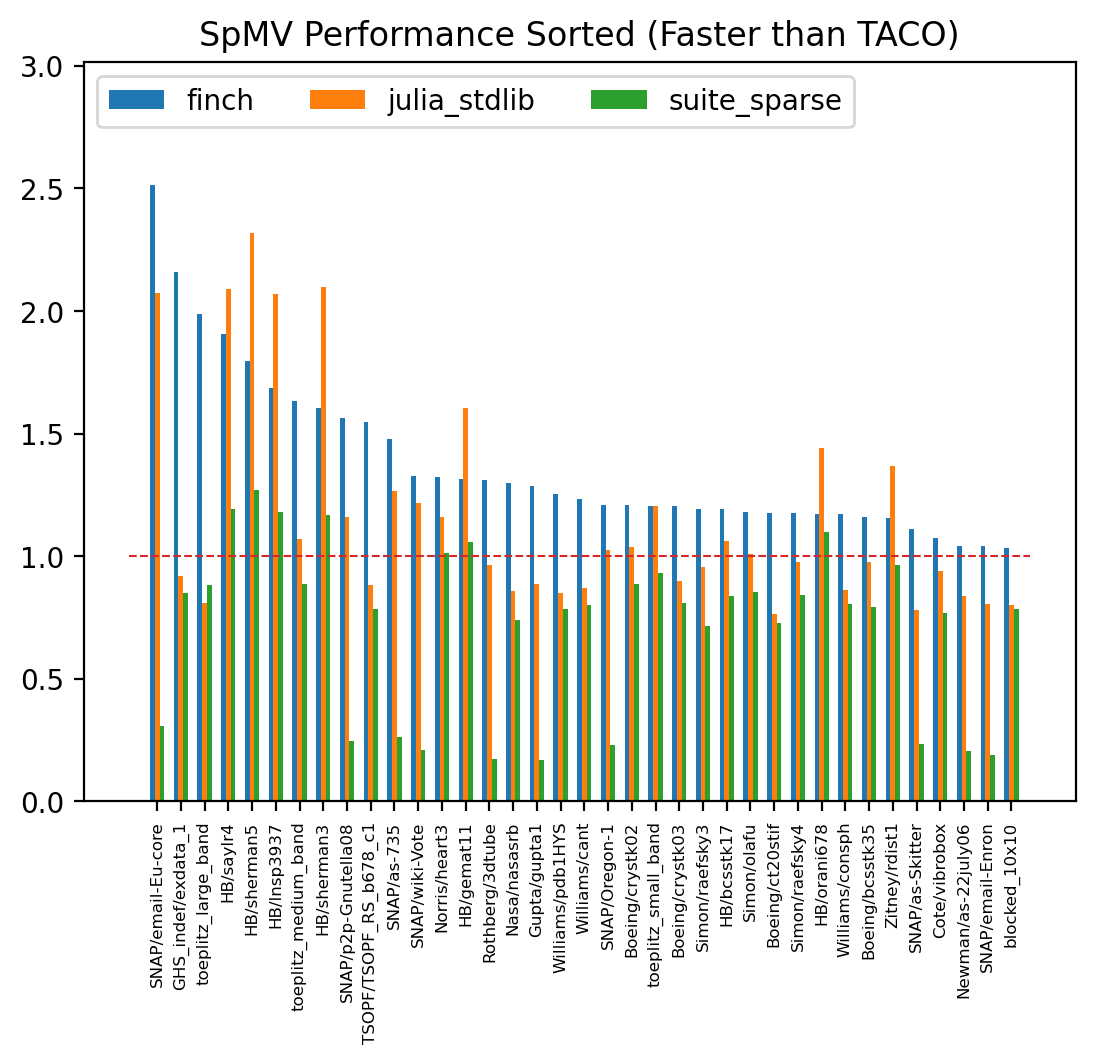
\includegraphics[width=\linewidth]{spmv_performance_sorted_(faster_than_taco).png}
    \end{minipage}%
    \begin{minipage}[t]{0.5\textwidth}
        \vspace{0pt} % Add this to ensure top alignment within minipage
        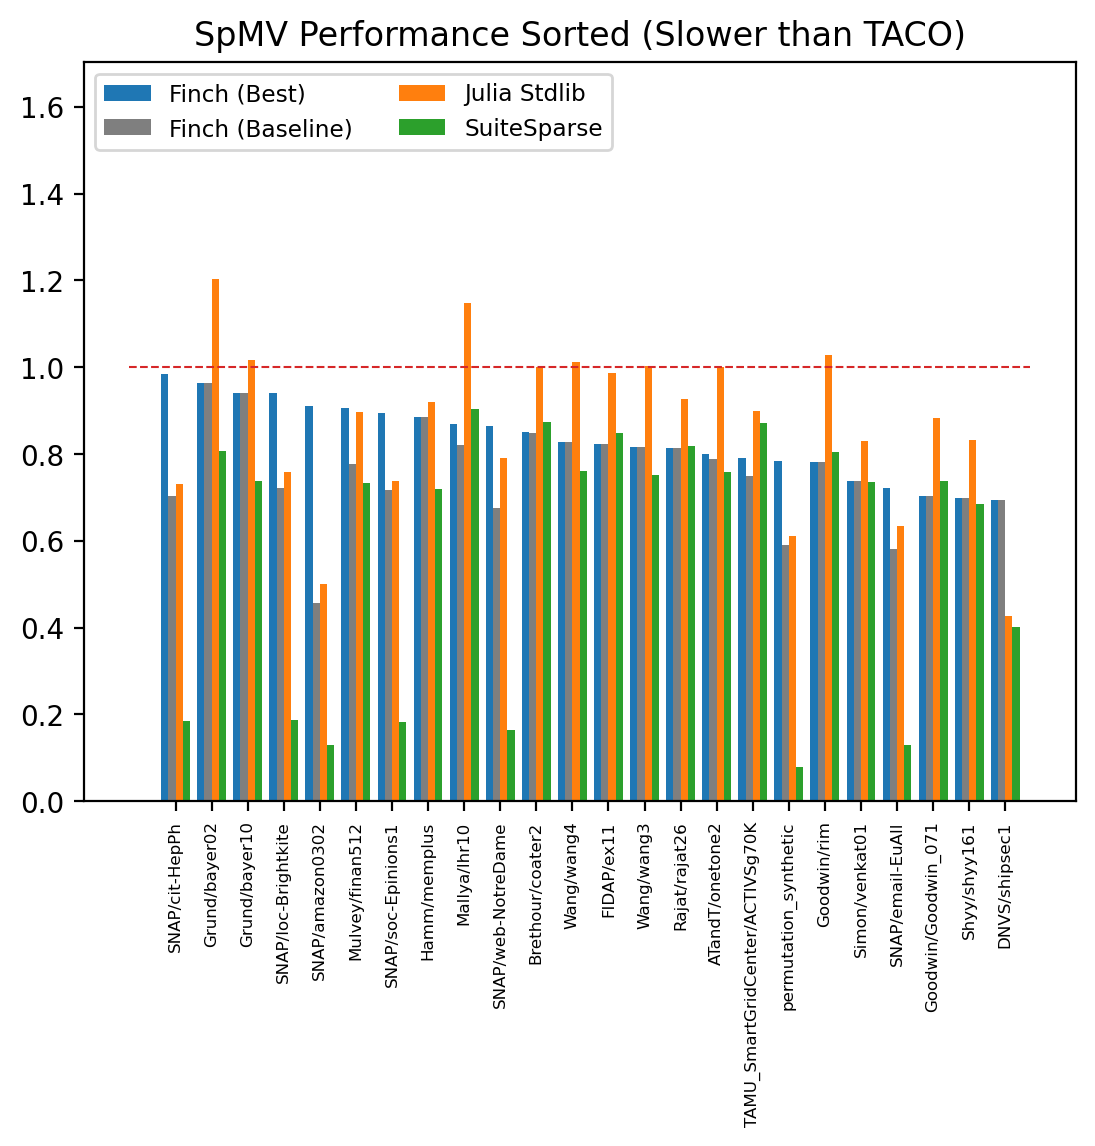
\includegraphics[width=\linewidth]{spmv_performance_sorted_(slower_than_taco).png}
    \end{minipage}
    \caption{Performance of SpMV across various tools.}
\end{figure}



\subsection{Programming over flexible data}

\subsubsection{RLE Blur}

-Compare against the zip/unzip version

- Which Datasets? Check taco-rle or looplets.
(perhaps consider if a neural network is the right call here)

\subsubsection{Histogram}


\subsubsection{Graph Applications}
\begin{figure}
	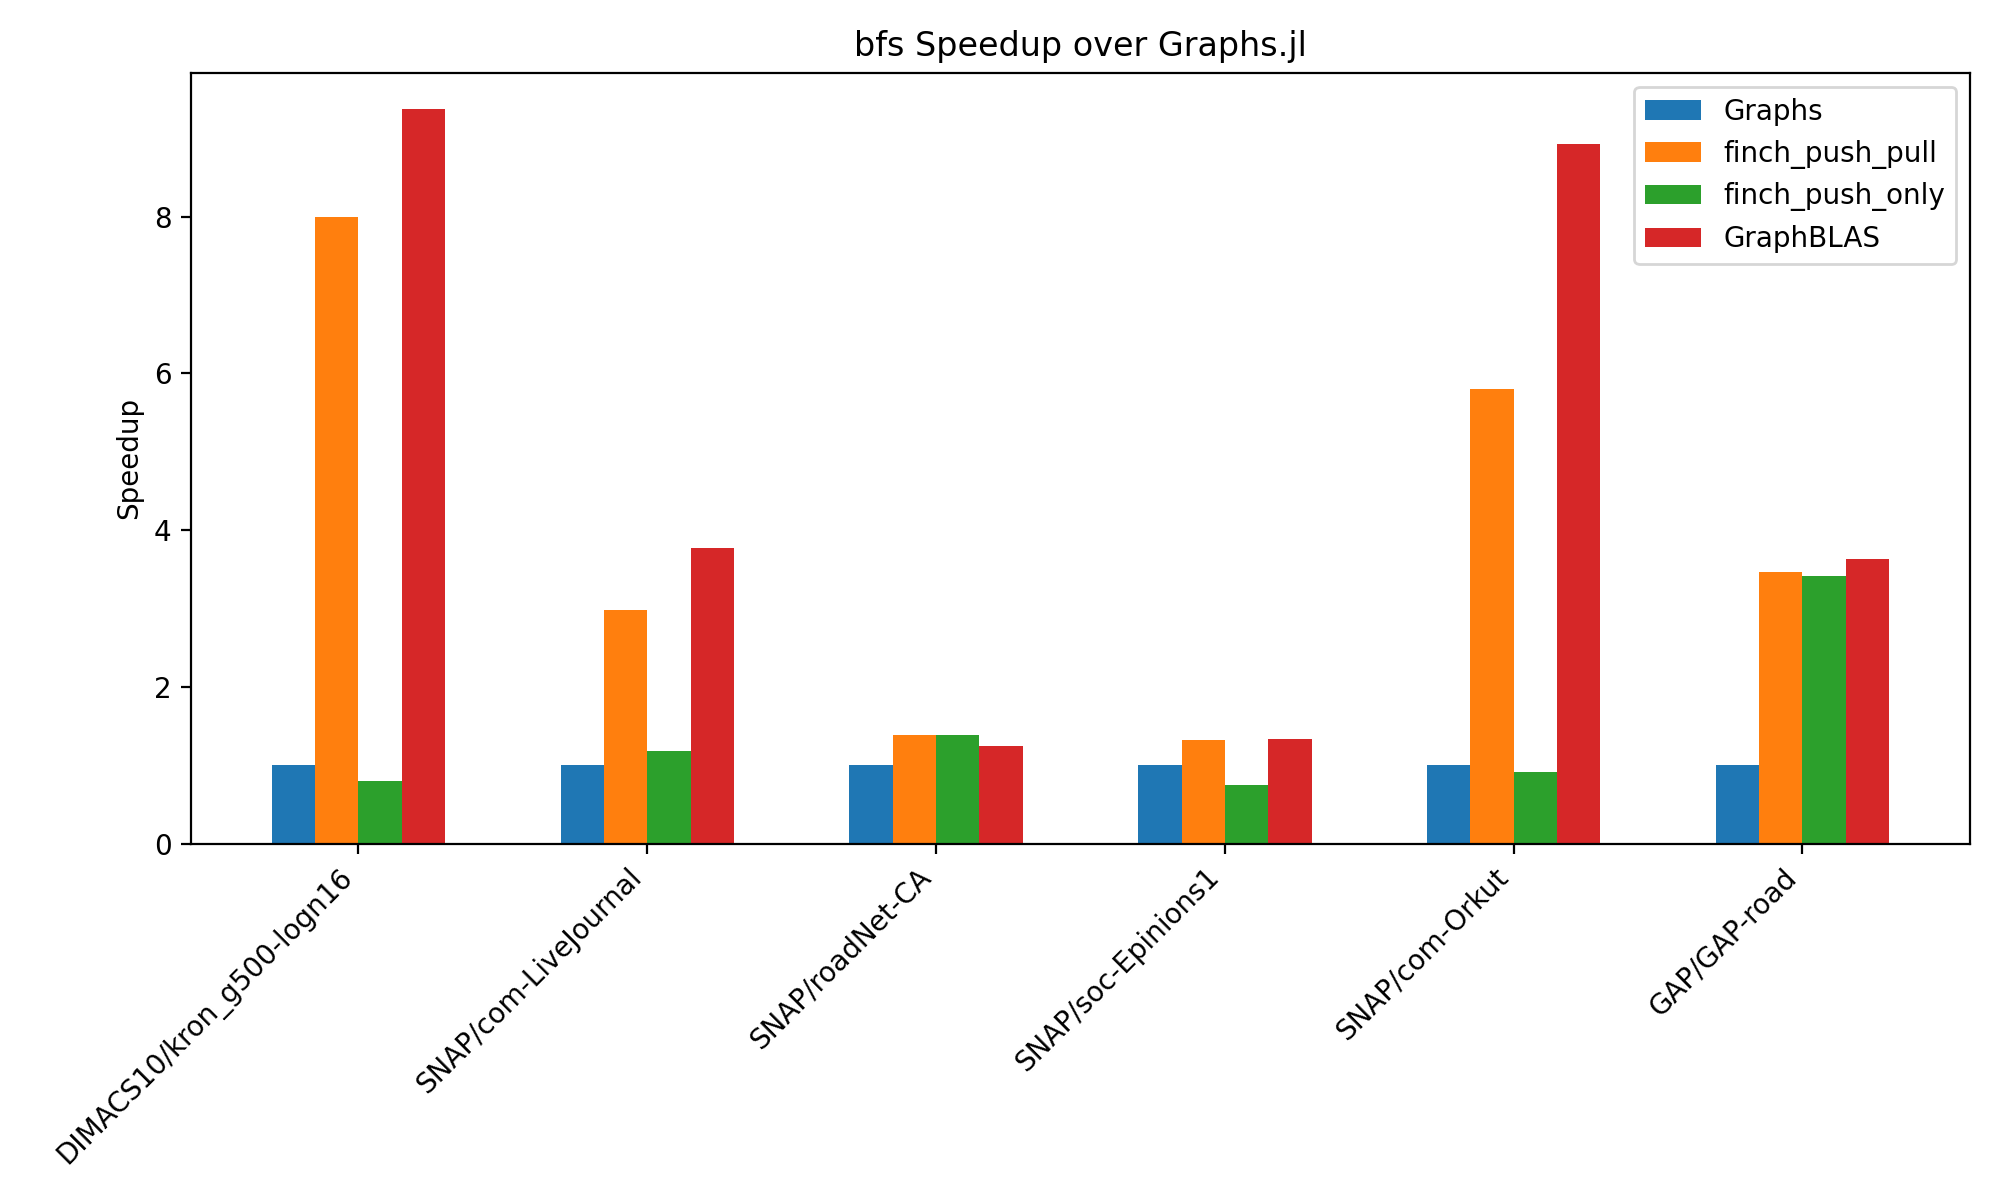
\includegraphics[width=\linewidth]{bfs_speedup_over_graphs.jl.png}
	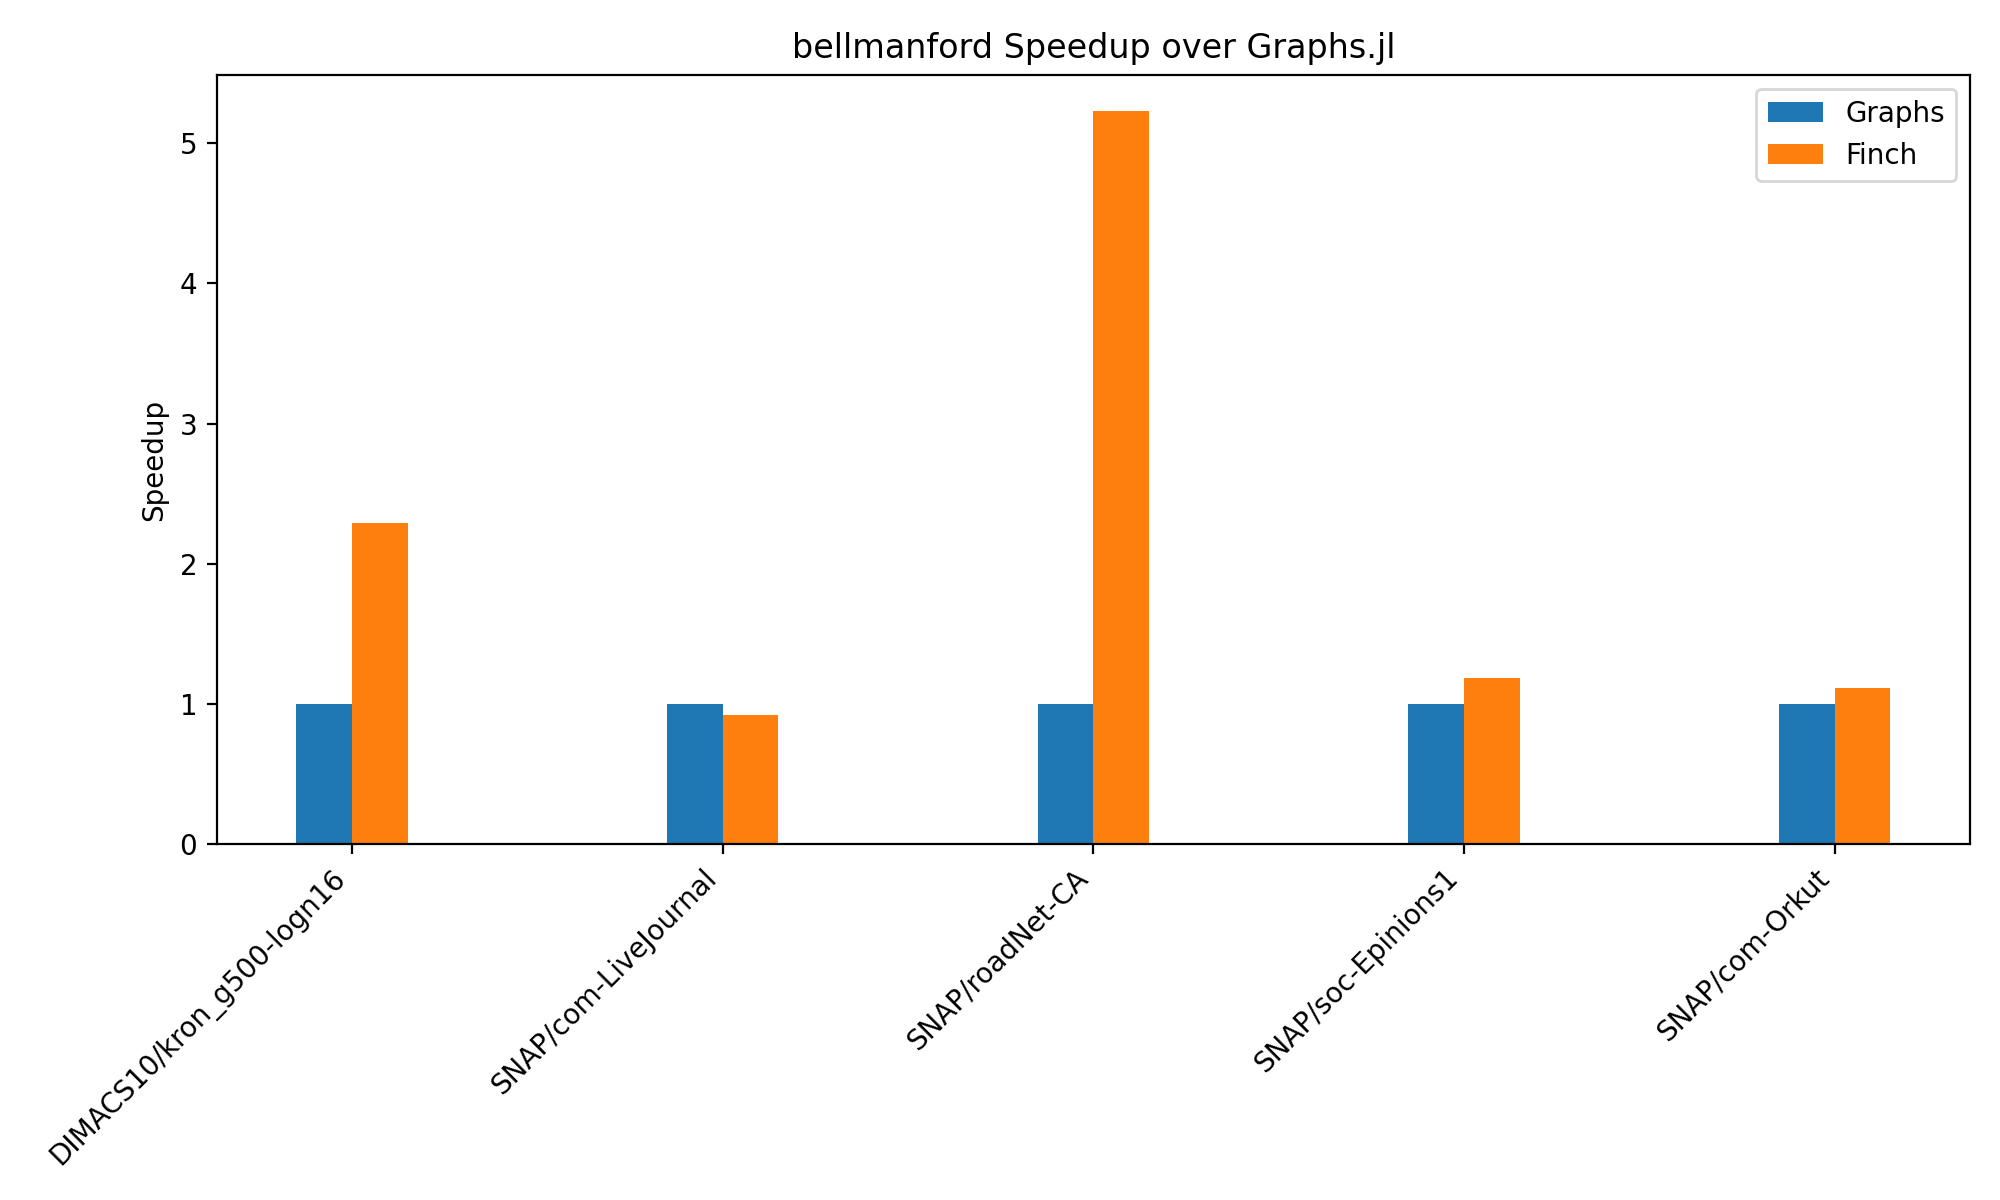
\includegraphics[width=\linewidth]{bellmanford_speedup_over_graphs.jl.png}
    \caption{Performance of graph apps across various tools.}
\end{figure}

\subsubsection{High-level kernel fusion}
Find an example where fusing the python interface gives a big speedup over non-fused kernels.

\bibliographystyle{alpha}
\bibliography{bibliography}

\end{document}